\section{Overall Structure}
In essence, our system is to reorganize the search log according to the structure of concepts and use the reorganized
structure to quickly retrieve the matching historical queries and return them to user.

In order to achieve that, we divide our system into two parts. One is the offline part, responsible for precomputing the
index of search log. The other one is the online part, which can retrieve the index, rank the candidate queries and show
 results. As is shown in Fig. \ref{fig:overall-structure}, the two part is connected by the index of search log.

\begin{figure}[h]
\centering
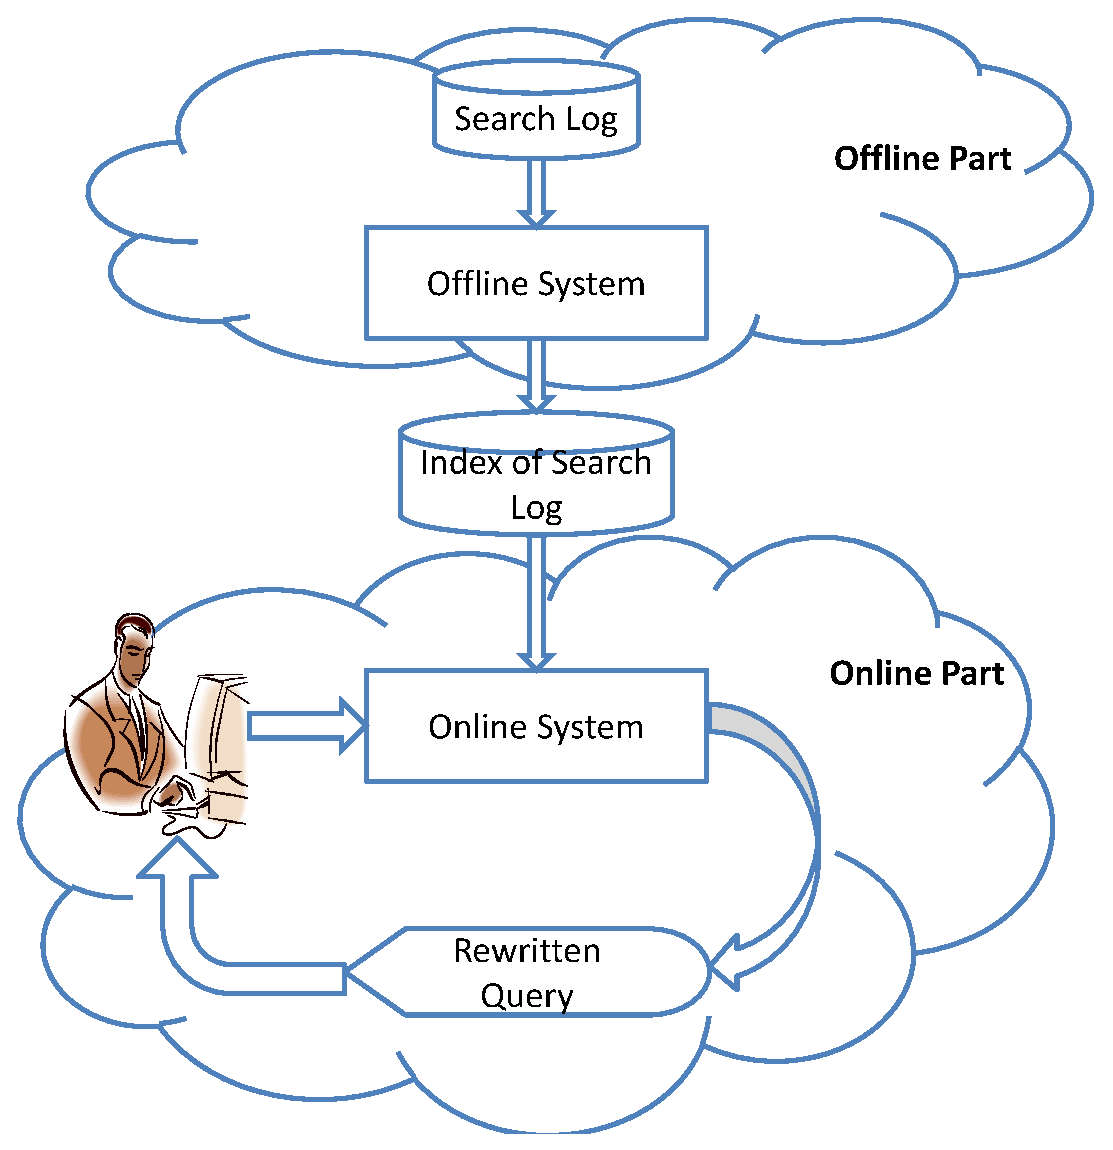
\includegraphics[scale=0.3]{images/overall}
\caption{Overall Structure of System}
\label{fig:overall-structure}
\end{figure}